% === Begin Label Data ===
% ID: 838
% 难度星级: 
% 标签: 
% 备注: 
% 组卷引用次数: 0
% === End  Label Data ===

\begin{problem}{2019}{G}{北京卷（文）}{8}{解析几何}
如图，$A,B$是半径为 $2$ 的圆的定点，$P$ 为圆周上的动点，$\angle APB$ 是锐角，大小为 $\beta$，图中阴影区域的面积的最大值为 (\hspace{1cm})
\begin{choices}
\choice{{ $4\beta+4\cos\beta$ }}
\choice{{ $4\beta+4\sin\beta$ }}
\choice{{ $2\beta+2\cos\beta$ }}
\choice{{ $2\beta+2\sin\beta$ }}
\end{choices}

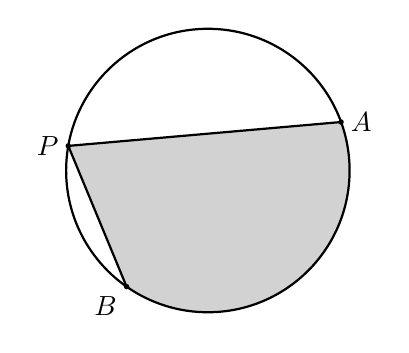
\begin{tikzpicture}[line cap=round,line join=round,scale=0.9]
\usetikzlibrary{calc}

\def\R{2.0}
\def\angA{20}
\def\angP{170}
\def\angB{235}

\coordinate (O) at (0,0);
\coordinate (A) at ({\R*cos(\angA)},{\R*sin(\angA)});
\coordinate (P) at ({\R*cos(\angP)},{\R*sin(\angP)});
\coordinate (B) at ({\R*cos(\angB)},{\R*sin(\angB)});

% 阴影：P--A--(沿不经过P的弧AB)--B--P
\path[fill=gray!35]
  (P) -- (A)
  arc[start angle=\angA,end angle=\angB-360,radius=\R]
  -- (P) -- cycle;

% 圆周
\draw[thick] (O) circle (\R);

% 弦
\draw[thick] (P)--(A);
\draw[thick] (P)--(B);

% 标注
\fill (A) circle (1.1pt) node[right] {$A$};
\fill (P) circle (1.1pt) node[left] {$P$};
\fill (B) circle (1.1pt) node[below left] {$B$};

\end{tikzpicture}
\end{problem}

\begin{answer}
B
\end{answer}

\begin{solutions}
考虑特殊情况，令 $\beta\to\dfrac{\pi}{2}$，此时阴影区域面积最大值接近 $4+2\pi$，只有 B 满足。

常规做法如下：

% 图2（解析右下）：圆心 O，点 A,B,D,P 在圆上，连线与虚线（示意）
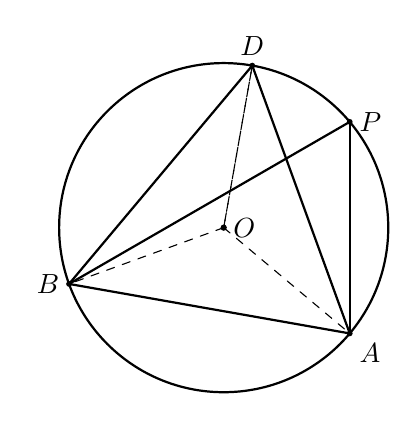
\begin{tikzpicture}[line cap=round,line join=round,scale=0.95]
\usetikzlibrary{calc}

\coordinate (O) at (0,0);
\def\R{2.2}

% points (choose angles to match the picture layout)
\coordinate (B) at ({\R*cos(200)},{\R*sin(200)});
\coordinate (A) at ({\R*cos(320)},{\R*sin(320)});
\coordinate (D) at ({\R*cos(80)},{\R*sin(80)});
\coordinate (P) at ({\R*cos(40)},{\R*sin(40)});

% circle
\draw[thick] (O) circle (\R);

% solid chords
\draw[thick] (B)--(A);
\draw[thick] (B)--(D);
\draw[thick] (D)--(A);
\draw[thick] (A)--(P);
\draw[thick] (B)--(P);

% dashed radii / helpers
\draw[dashed] (O)--(A);
\draw[dashed] (O)--(B);
\draw[dashed] (O)--(D);
\draw[dashed] (D)--(O);

% center mark
\fill (O) circle (1.2pt) node[right] {$O$};

% point marks + labels
\fill (A) circle (1.1pt) node[below right] {$A$};
\fill (B) circle (1.1pt) node[left] {$B$};
\fill (D) circle (1.1pt) node[above] {$D$};
\fill (P) circle (1.1pt) node[right] {$P$};

\end{tikzpicture}

设弧 $\widehat{AB}$ 与线段 $AB$ 围成的弓形面积为 $S$，显然 $S$ 为定值，当 $S_{\triangle ABP}$ 最大时，阴影区域面积最大。又当 $P$ 运动到点 $D$ 位置时，$S_{\triangle ABP}$ 面积最大，因此阴影区域面积的最大值即为 $S_{\triangle AOD}+S_{\triangle BOD}+S_{\text{扇}AOB}=2S_{\triangle AOD}+S_{\text{扇}AOB}$.

$\angle BOD=\angle AOD=\pi-\beta$，$\angle AOB=2\beta$，

$2S_{\triangle AOD}+S_{\text{扇}AOB}
=2\cdot\dfrac{1}{2}\cdot2^{2}\cdot\sin(\pi-\beta)+\dfrac{1}{2}\cdot2\beta\cdot2^{2}
=4\sin\beta+4\beta$

选 B.
\end{solutions}